
\chapter{Validation}
\section{Validation Strategy}
Model validation could be considered an important step towards creating a robust and useful simulation tool. A greater volume of literature is availalbe for the validation of Ray based methods such as~\cite{Ahnert2005,Tsingos2002,Foteinou2010}, and the validation of a hybrid scheme by Southern \textit{et al} is available ~\cite{Southern2013}. Studies such as Hill~\cite{Hill2012} incorporate validation as a subset of a greater work. This section will review the results of simulations using the FDTD and PSTD tools described above, with a small 3D domain and different excitation signals. The validation of these simulation tools will be in proving that wave propagation is occurring.\\

\subsection{The Domain}
The domain used was a fully bounded rectangular room with the following properties:\\

\begin{itemize}
\item Length $L_x = 5m$
\item Width $L_x = 4m$
\item Height $L_z = 3m$
\item Volume = $ v = 60m^3$
\item Surface Area $S_{area} = 94m^2$
\item Uniform Absorption Coefficient $\alpha = 0.45 $
\item Schroeder Frequency  $f_{schroeder} = 107Hz $,
\item The Reflection Order $N_{reflections} = 30.7$
\item Mean Free Path Between Reflections $MFP = 2.55m$
\item Eyring Reverberation Time $RT_{60} = 0.1719s $
\end{itemize}

The theoretical room mode frequencies below the Schroeder frequency are shown below:\\
\begin{figure}[H]
\centering
  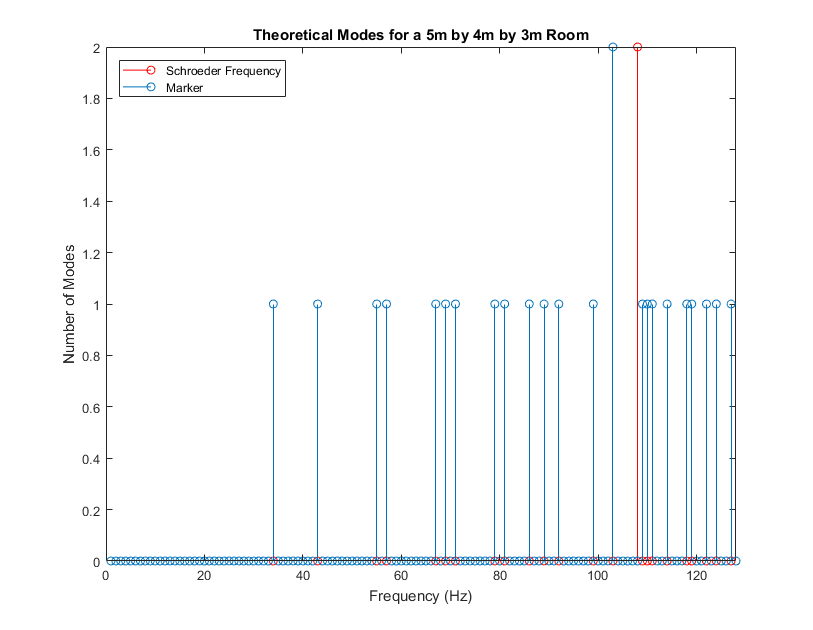
\includegraphics[width=\textwidth]{./graphics/modesuptoschr.png}
  \caption{Room Modes up to Schroeder Frequency for a Small Rectangular Room}
\end{figure}

The source position was $1.0m$ in each direction from a bottom cornerl. Five receiver positions were recorded, one quater on the x and y dimensions from each corner, all at the middle of the domain on the z axis. The source type was a soft source as described earlier in this doccument. Two source signals were implemented in seperate simulations; an MLS sequence of 11th order with 2 repetitions, and a $1kHz$ tone burst signal containing three pulses of 10 cycles with a gap of equal length to the bursts. The MLS signal was generated using the MLS toolbox by Mark Thomas~\cite{Mrt2008}, and the tone-burst was generated using tools in the Matlab DSP Systems toolbox. The signals were normalised with a Gaussian window to the length of the signals. The maximum frequency of interest in this validation was $5kHz$, giving a $0.333e^{-5}$ step time for the FDTD and SFDTD simulation, and a $0.1e^{-4}$ step time for the PSTD simulation.

\section{Results}
The aim of the simulations was be to show that the models propagate pressure waves with minimal error in the average power spectral density between source and receiver location. Frequency domain averaging of the source and receiver location signals was undertaken using Matlab pwelch function. This function uses Welch's overlapping segment averaging estimator to average a series of discrete Fourier transforms, creating a smoothed average frequency response over the course of the signal without transforming the whole signal in one go~\cite{Welch1967}.

\subsection{FDTD Simulation Results}

\begin{figure}[H]
\centering
\textbf{FDTD Validation Data}
  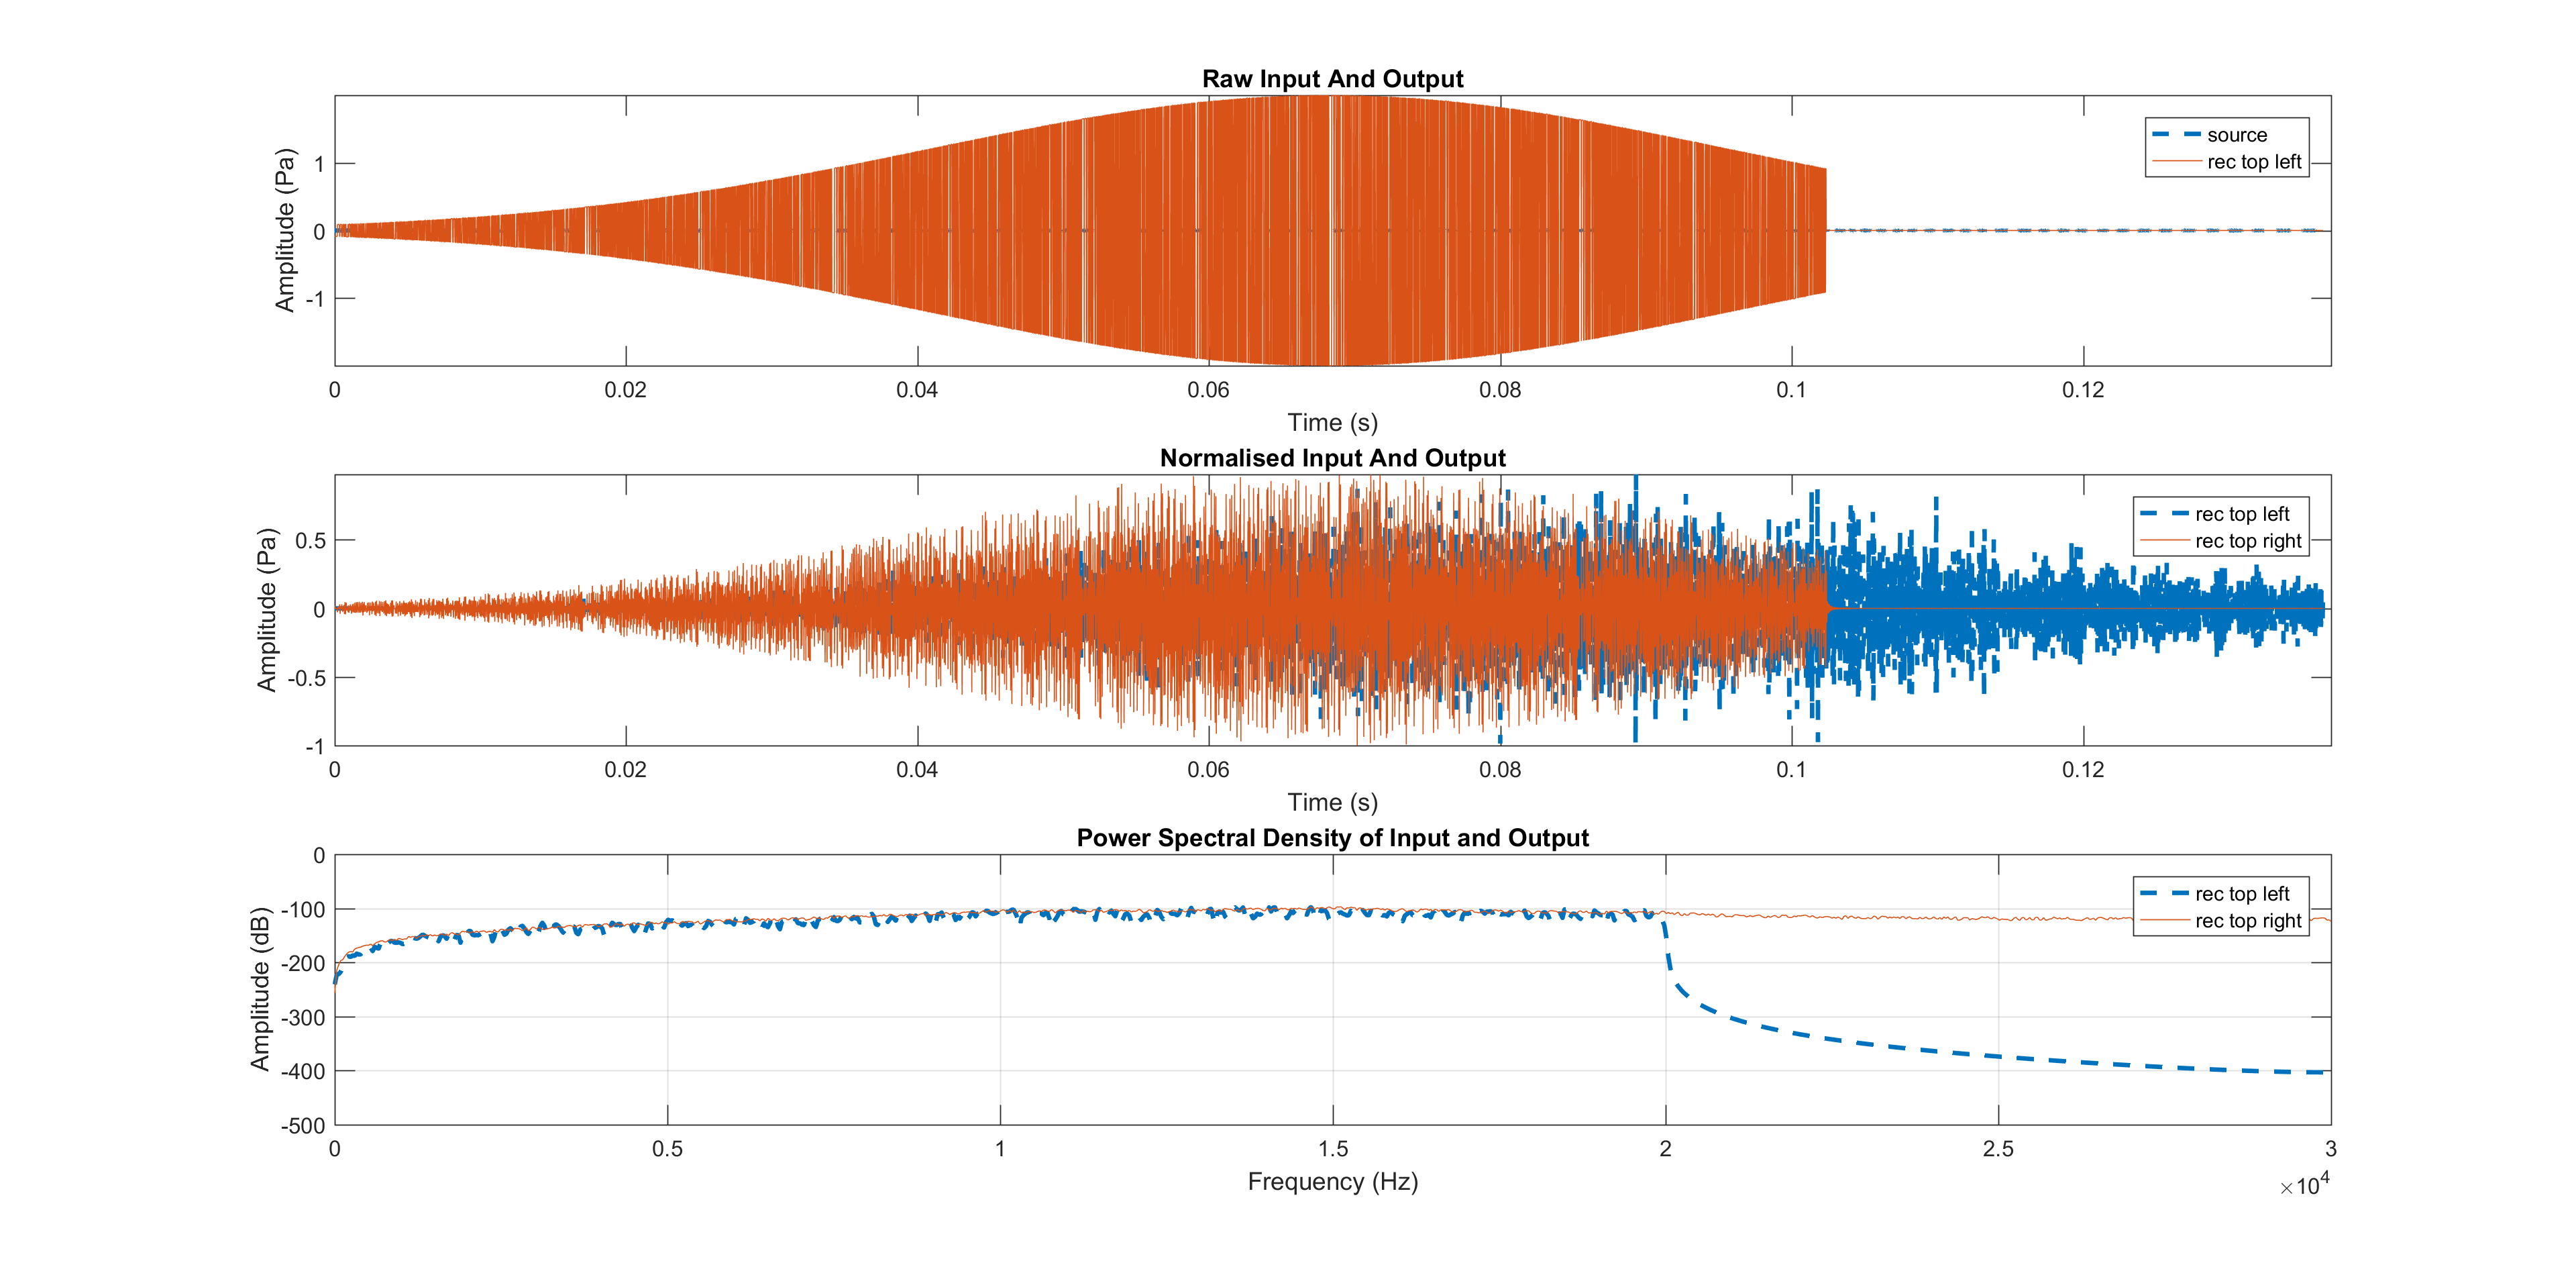
\includegraphics[width=\textwidth]{./graphics/FDTDvalidationFinal.png}
  \caption{Validation data of FDTD simulation}
\end{figure}

\subsection{SFDTD Simulation Results}

Results

\subsection{PSTD Simulation Results}
\begin{figure}[H]
\centering
\textbf{PSTD Validation MLS Data}
  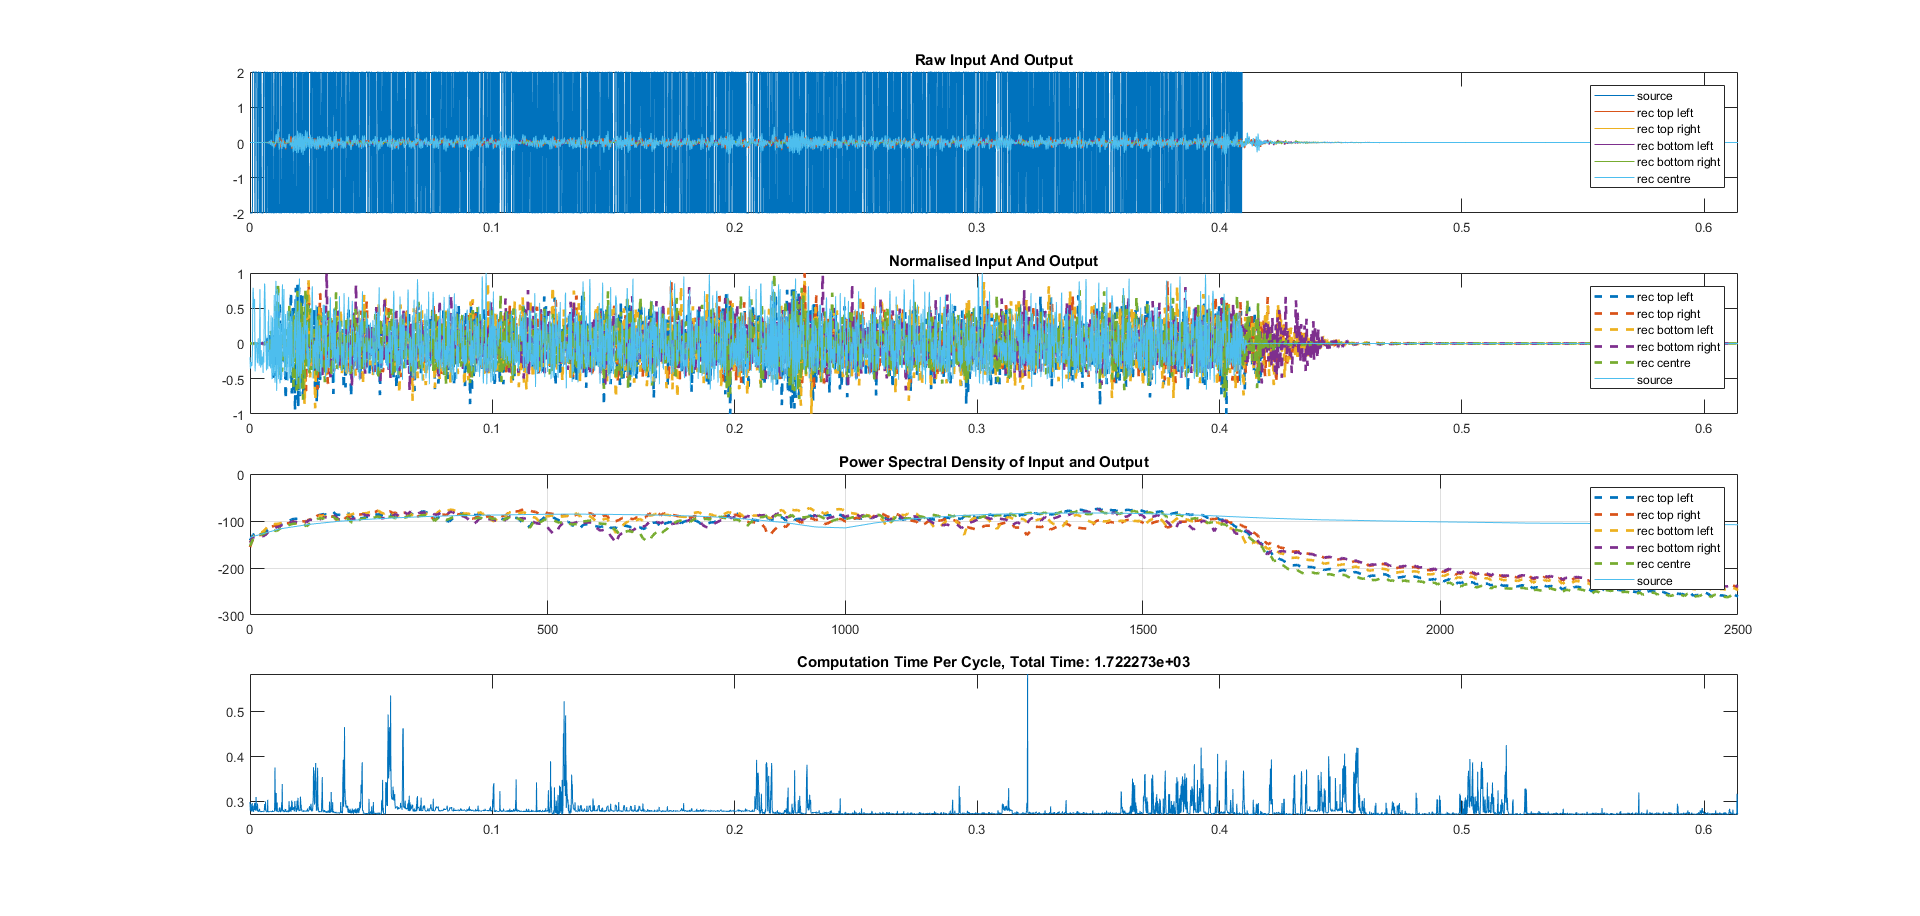
\includegraphics[width=\textwidth]{./graphics/PSTDvalidationFinal.png}
  \caption{Validation data of PSTD simulation With MLS Source}
  \textbf{PSTD Validation Tone Burst Data}
  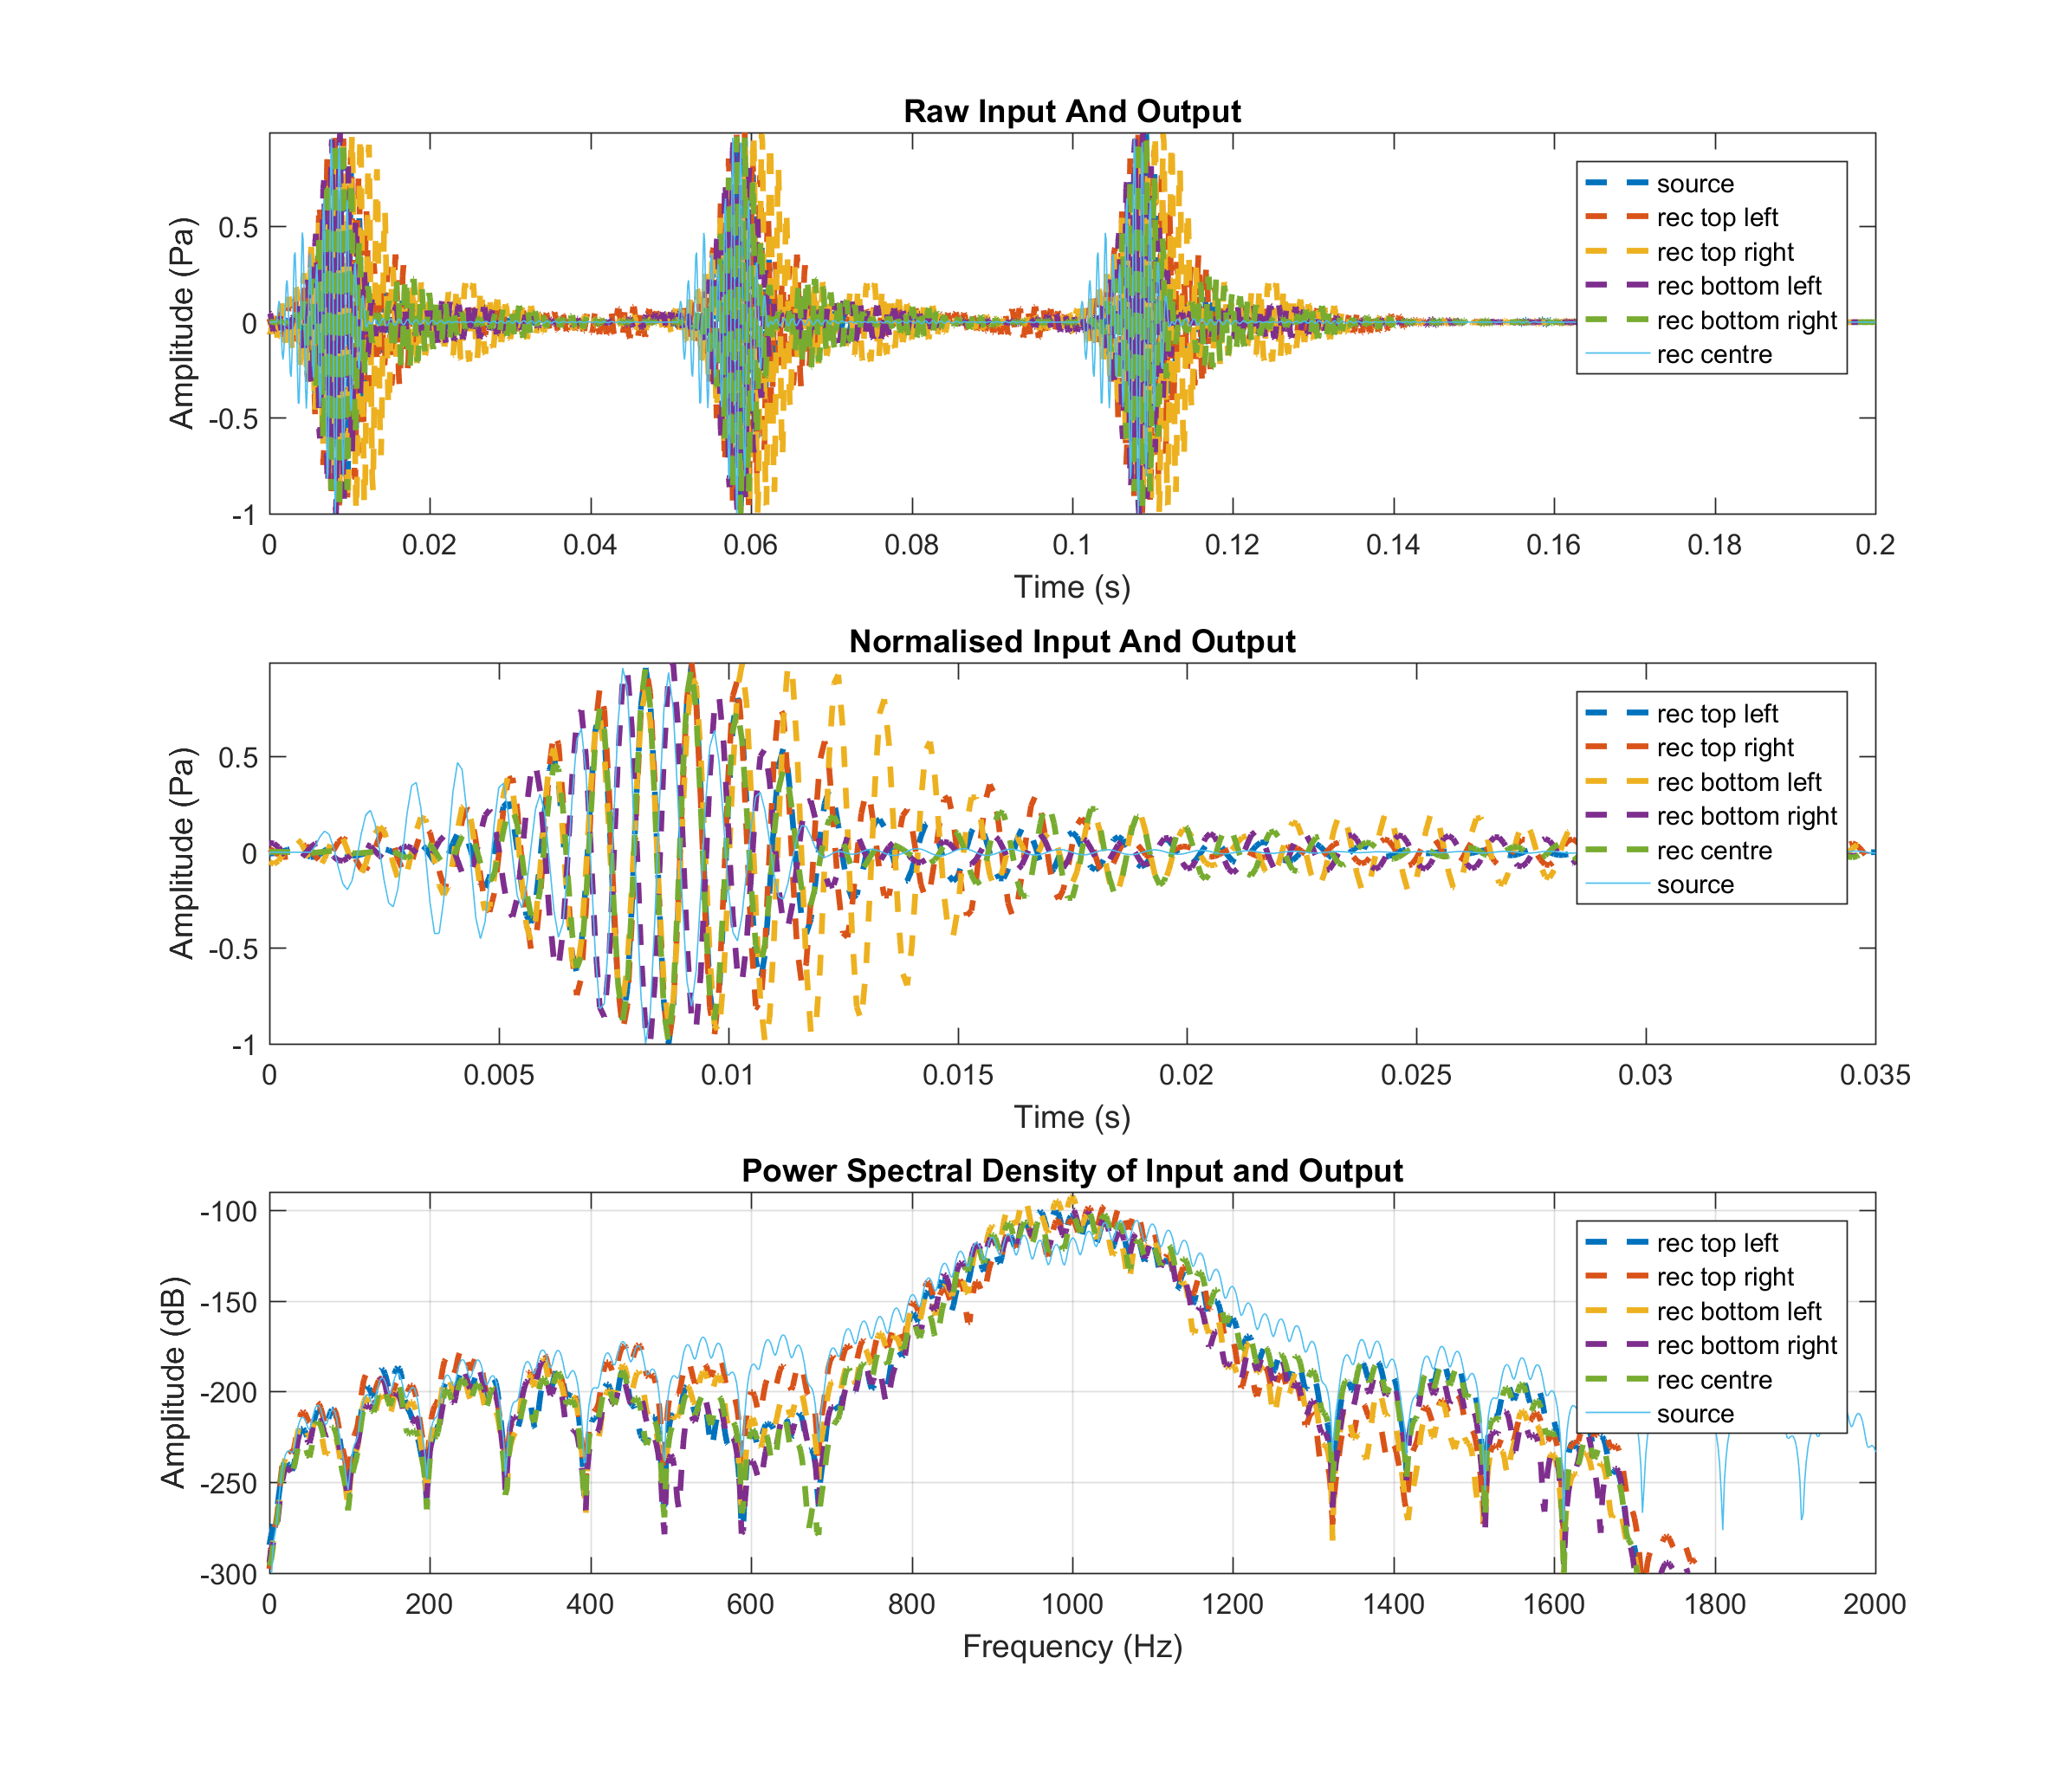
\includegraphics[width=\textwidth]{./graphics/PSTDvalidationFinalTB.png}
  \caption{Validation data of PSTD simulation With Tone Burst Source}
\end{figure}

It can be seen that both simulations have reasonably good agreement between the power spectral densities (PSD) of the source and receivers in the frequency region of interest. There is a significant low frequency signal present in the PSTD response, in both the source and receiver sections.  Due to the 6 steps per wavelength of the FDTD simulation, the time step was also smaller than for the PSTD simulation. As such when using Matlabs Pwelch function to perform PSD estimation, the estimation was made beyond the frequency range of interest.\\


\section{Validating The SFDTD Method}
As the SFDTD method was implemented only to 2D and it could not be validated with the 3D FDTD and PSTD methods as above. The SFDTD method was tested using a 5m by 4m domain, with absorption coefficients of $ \alpha = 0.45$. The signal used was a chirp that was generated using the Chip function of the Matlab DSP Systems Toolbox, with a start frequency of 100Hz and a stop frequency of half the maximum target frequency (or a quarter of Nyquist), that was normalised to $100dBSPL$ and has a sweep time of $0.4s$. Before normalisation, a Hamming window was applied to the signal to minimize the discontinuity of introducing the source. The figure below presents the output data for the SFDTD validating simulation:\\

\begin{figure}[H]
\centering
\textbf{SFDTD Validation Data}
  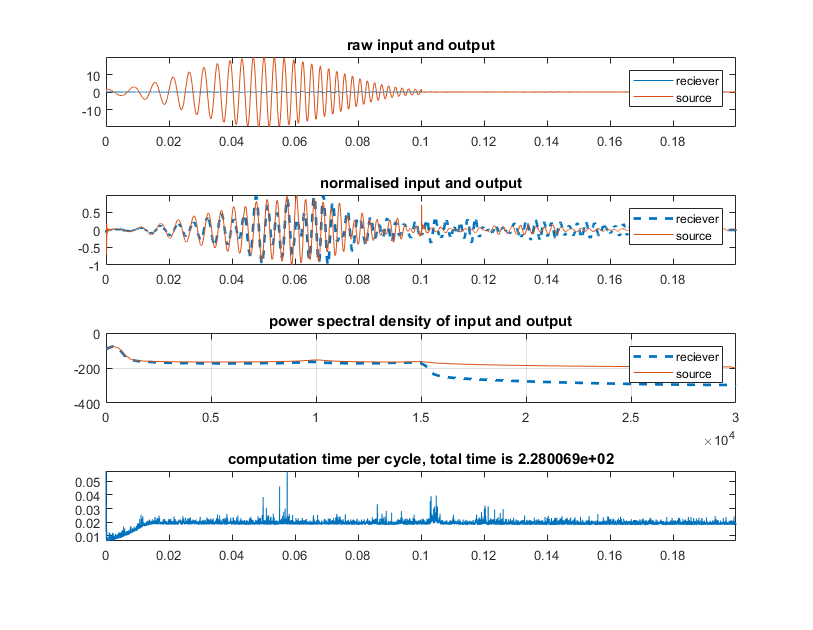
\includegraphics[width=\textwidth]{./graphics/SFDTDvalidationFinal.png}
  \caption{Validation data of PSTD simulation}
\end{figure}
As with the PSTD method there is a shared low frequency component, but the PSD between source and receiver are very close to well beyond the highest frequency of interest.